%% IEEE double-column conference report
%% Compile:  pdflatex report.tex ; bibtex report ; pdflatex report.tex ; pdflatex report.tex
%% (or upload the report/ folder to Overleaf and press Recompile)
\documentclass[conference]{IEEEtran}
\IEEEoverridecommandlockouts
\usepackage{cite}
\usepackage{amsmath,amssymb,amsfonts}
\usepackage{graphicx}
\usepackage{booktabs}
\usepackage{array}
\usepackage{url}
\usepackage{pifont}
\usepackage{xcolor}
\usepackage[hidelinks]{hyperref}
\graphicspath{{../figures/}}

%% ---- Result macros (update from results/metrics.json after a full run) ----
% External (cross-dataset, deepset) F1 scores
\newcommand{\FiLR}{0.21}
\newcommand{\FiSVM}{0.28}
\newcommand{\FiRF}{0.60}
\newcommand{\FiXGB}{0.61}
\newcommand{\FiTF}{0.28}

\begin{document}

\title{Real-Time Detection of Prompt Injection Attacks Against
LLM-Integrated REST APIs Using a Comparative Machine Learning Pipeline}

\author{\IEEEauthorblockN{[Your Full Name (as per NCI records)]}
\IEEEauthorblockA{\textit{MSc in Artificial Intelligence} \\
\textit{National College of Ireland}\\
Dublin, Ireland \\
Student No.: [xxxxxxxx] \\
[your.email]@student.ncirl.ie}}

\maketitle

\begin{abstract}
Prompt injection is ranked LLM01 in the 2025 OWASP Top~10 for LLM
applications, yet most published detectors are validated on a single dataset
and rarely report the inference latency that an inline production guardrail
demands. This project builds and critically compares three families of
prompt-injection detectors intended to sit as a screening layer in front of an
LLM-integrated REST API: (i)~an interpretable, low-latency TF-IDF baseline with
Logistic Regression and a calibrated Linear SVM; (ii)~sentence-embedding
classifiers (\texttt{all-MiniLM-L6-v2}) feeding Random Forest and XGBoost; and
(iii)~a fine-tuned transformer encoder. Models are trained on the
\emph{ahsanayub/malicious-prompts} and \emph{SPML} corpora
(\(\approx\!28\text{k}\) prompts) and stress-tested on the unseen
\emph{deepset} corpus to quantify \emph{cross-dataset} generalisation. We
evaluate accuracy, precision, recall, F1, ROC-AUC, stratified 5-fold
cross-validation, confusion matrices, per-request latency, and model
explainability. The study shows that lexical baselines are fastest and dominate
in-distribution but transfer poorly to novel attacks, whereas embedding-based
models generalise best across datasets, exposing an accuracy/latency/robustness
trade-off that is central to real-world deployment.
\end{abstract}

\begin{IEEEkeywords}
prompt injection, LLM security, API security, machine learning, text
classification, cross-dataset generalisation
\end{IEEEkeywords}

\section{Introduction}
Large Language Models (LLMs) are increasingly exposed through REST APIs and
micro-services. The OWASP Gen~AI Security Project ranks \emph{Prompt Injection}
as the top risk (LLM01:2025) for such applications, noting that
retrieval-augmented generation and fine-tuning cannot fully prevent it because
the model itself cannot reliably separate trusted instructions from untrusted
user content~\cite{owasp2025}. The threat is not confined to the model:
Pedro~\emph{et al.}\ demonstrate that a prompt injection can be escalated into a
classical SQL injection against the backend database through LangChain
middleware, and that input/output guardrails add measurable
overhead~\cite{pedro2025prompt}. Prompt injection is therefore an
\emph{API-security} problem, and a practical defence must be both accurate and
fast enough to run inline on every request.

This work is motivated by industry experience operating .NET REST APIs and
micro-services serving tens of thousands of monitored requests per day, where an
additional per-request control must add only a few milliseconds. We frame
prompt-injection detection as a supervised text-classification task placed as a
screening layer immediately before the LLM call.

\textbf{Research question.} \emph{To what extent can lightweight
embedding-based and transformer-based classifiers detect prompt-injection
attempts when deployed as a screening layer in front of an LLM-integrated REST
API, and what is the trade-off between detection accuracy, interpretability, and
per-request latency required for production deployment?}

\textbf{Objectives.} (1)~Implement three method families spanning the
simplicity/expressiveness spectrum; (2)~train on two corpora and evaluate on a
\emph{third, unseen} corpus to measure cross-dataset robustness --- a gap
identified in the literature; (3)~profile per-request latency to assess
deployability; and (4)~provide explainability and a critical ethical analysis.

\textbf{Contributions.} We contribute a reproducible, latency-aware comparison
of five detectors under a strict cross-dataset protocol, an explainability
analysis linking lexical features to attack patterns, and a working FastAPI
screening service that operationalises the best model. Sections~\ref{sec:related}
--\ref{sec:conclusion} cover related work, methodology, evaluation, ethics,
results, and conclusions.

\begin{figure}[t]
\centering
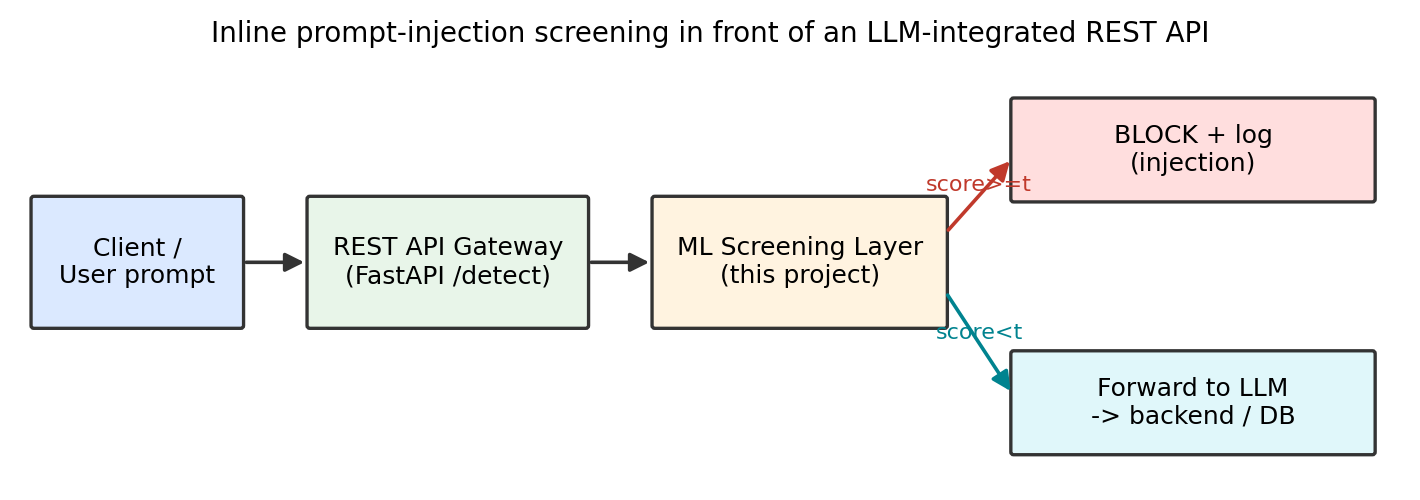
\includegraphics[width=\columnwidth]{fig0_architecture.png}
\caption{Proposed deployment. Each user prompt is screened by the ML layer at
the API gateway \emph{before} it reaches the LLM: prompts scoring above a
tunable threshold~$t$ are blocked and logged, the rest are forwarded. The
detector must therefore be both accurate and low-latency.}
\label{fig:arch}
\end{figure}

\section{Related Work}\label{sec:related}
Recent research treats prompt-injection detection as a natural-language
processing problem. Ayub and Majumdar~\cite{ayub2024embedding} compare three
embedding models and find that classical algorithms such as Random Forest and
XGBoost outperform neural baselines, indicating that lightweight models can be
both effective and cheap---attractive for an API gateway. However, they do not
report inference time, leaving the deployment cost unquantified; our study adds
exactly this latency dimension and reuses their embedding-classifier design as a
baseline to extend.

Rahman~\emph{et al.}~\cite{rahman2024multilingual} pair multilingual BERT
embeddings with Gaussian Na\"ive Bayes, Random Forest, SVM, and Logistic
Regression, concluding that \emph{embedding quality matters more than classifier
complexity}. Their evaluation is confined to a single dataset, so cross-dataset
transfer---the core of our protocol---remains untested. Ji, Li and
Mao~\cite{ji2025detection} combine transformer semantic embeddings with
hand-crafted heuristic features and achieve high F1 across several LLMs; the
reliance on hand-crafted features, however, risks brittleness against unseen
attack phrasings, motivating our purely learned transformer variant.

Sharma, Gupta and Grossman~\cite{sharma2024spml} introduce the System Prompt
Meta Language (SPML) and a dataset of realistic system prompts paired with
labelled user prompts, framing injection relative to a defender's system
prompt---a realistic operational setting we adopt as a training corpus.
Pedro~\emph{et al.}~\cite{pedro2025prompt} show, practically, that injections can
cascade into SQL injection through middleware and that guardrails impose
overhead, reinforcing the need for a \emph{fast} inline detector. Finally,
Zhang~\emph{et al.}~\cite{zhang2025llmcyber} review over 300 studies of LLMs in
cybersecurity and conclude that realistic deployment concerns---latency and
integration with existing security infrastructure---remain under-explored.

\textbf{Synthesis and gap.} Collectively the literature establishes that both
classical and transformer approaches can detect injections and that embedding
quality is pivotal, but two gaps persist: (i)~single-dataset evaluation that
masks poor generalisation, and (ii)~the absence of latency reporting for inline
use. This project targets both gaps directly with a cross-dataset, latency-aware
comparison and a baseline-versus-advanced framing rather than a
state-of-the-art-only comparison. Table~\ref{tab:related} positions our work
against the closest studies.

\begin{table}[t]
\caption{Positioning against closely related work. CD = cross-dataset
evaluation; Lat.\ = reports inference latency.}
\label{tab:related}
\centering
\small
\begin{tabular}{@{}lccc@{}}
\toprule
Study & Methods & CD & Lat. \\
\midrule
Ayub \& Majumdar~\cite{ayub2024embedding}   & Embeddings + RF/XGB & \ding{55} & \ding{55} \\
Rahman \emph{et al.}~\cite{rahman2024multilingual} & mBERT + 4 classifiers & \ding{55} & \ding{55} \\
Ji \emph{et al.}~\cite{ji2025detection}     & Transformer + heuristics & partial & \ding{55} \\
Sharma \emph{et al.}~\cite{sharma2024spml}  & SPML DSL + LLM & \ding{55} & \ding{55} \\
\textbf{This work} & \textbf{TF-IDF + Emb.\ + Transformer} & \checkmark & \checkmark \\
\bottomrule
\end{tabular}
\end{table}

\section{Methodology}\label{sec:method}
\subsection{Datasets and unification}
We use three publicly available corpora (Table~\ref{tab:data}), accessible
without restriction from Hugging Face. The \emph{ahsanayub/malicious-prompts}
corpus~\cite{ahsandataset} ($\approx$467k prompts, $\sim$23.5\% malicious) is the
large primary source; we take a reproducible stratified subsample to keep the
CPU pipeline tractable. The \emph{SPML} corpus~\cite{spmldataset} contributes
16k labelled user prompts. The \emph{deepset} corpus~\cite{deepsetdataset}
(662 prompts) is reserved \emph{entirely} as the unseen cross-dataset test set
and never used for training or tuning. All sources are unified to a common
\{\texttt{text}, \texttt{label}\} schema (SPML uses the user prompt), cleaned
(whitespace normalisation, null removal), de-duplicated, and any train rows
overlapping the external test are removed to prevent leakage. The full ahsan CSV
(467k rows) ships with the artefact; only the \emph{training} subsample is
reduced for CPU tractability, and the sample size is a single configuration
constant that can be raised on more capable hardware.

\begin{table}[t]
\caption{Datasets after cleaning and de-duplication.}
\label{tab:data}
\centering
\small
\begin{tabular}{@{}lrrl@{}}
\toprule
Corpus & Prompts & \% Injection & Role \\
\midrule
ahsanayub (sampled) & $\sim$12{,}000 & 23.5 & Train \\
SPML & $\sim$15{,}900 & 78.8 & Train \\
deepset & 662 & 39.7 & Unseen test \\
\bottomrule
\end{tabular}
\end{table}

\subsection{Data preparation and preprocessing}
Preprocessing is deliberately light so that the detector remains
attack-agnostic. Each prompt is lower-cased implicitly by the vectoriser,
control characters (e.g.\ NUL) are stripped, runs of whitespace are collapsed to
a single space, and empty strings are discarded. Exact duplicates are removed
\emph{within} each corpus (the ahsan corpus in particular contains repeated
templated prompts), and any training prompt whose text also occurs in deepset is
deleted to guarantee an untainted external test. Labels are coerced to integers
$\{0,1\}$ with malformed rows dropped. No stemming or stop-word removal is
applied, because injection cues (``ignore'', ``system'', ``instructions'') are
themselves common words whose \emph{combinations} carry signal. For the
embedding and transformer models the raw cleaned text is passed directly to the
respective tokenisers, so no manual feature construction is required.

\subsection{Feature engineering and models}
Three method families span the complexity spectrum, each justified by the
literature and by the deployment constraint.

\textbf{(1) Interpretable baseline.} A union of word (1--2 gram) and character
(3--5 gram, \texttt{char\_wb}) TF-IDF features feeds a Logistic Regression and a
calibrated Linear SVM. Character n-grams capture obfuscated tokens (e.g.\
``ig\-nore''), and the model is fully interpretable and sub-millisecond---ideal
for an inline gateway~\cite{pedregosa2011scikit}.

\textbf{(2) Sentence-embedding classifiers.} \texttt{all-MiniLM-L6-v2}
sentence embeddings~\cite{reimers2019sentencebert} (384-d, L2-normalised) feed a
Random Forest~\cite{breiman2001randomforest} and
XGBoost~\cite{chen2016xgboost}, replicating and extending
Ayub and Majumdar~\cite{ayub2024embedding}. Semantic embeddings should
generalise to paraphrased attacks that lexical models miss.

\textbf{(3) Fine-tuned transformer.} A pre-trained encoder is fine-tuned with a
classification head, following Ji~\emph{et al.}~\cite{ji2025detection}. We report
results with DistilBERT~\cite{sanh2019distilbert} as a CPU-efficient encoder; the
pipeline is architecture-agnostic and switches to the proposal's
DeBERTa-v3-base~\cite{he2021debertav3} via a single configuration flag when a GPU
is available.

\subsection{Imbalance handling, tuning, and validation}
Class imbalance is addressed with \texttt{class\_weight="balanced"} (linear
models, Random Forest), \texttt{scale\_pos\_weight} (XGBoost), and a weighted
cross-entropy loss (transformer). The baseline regularisation strength $C$ is
tuned by \texttt{GridSearchCV} (5-fold, F1). Validation is threefold: stratified
5-fold cross-validation on the training pool, an internal stratified hold-out
(20\%), and the external \emph{deepset} set. This layered design distinguishes
in-distribution fit from genuine cross-dataset robustness. Experiments use a
fixed seed (42) for reproducibility. Table~\ref{tab:hyper} lists the key
hyper-parameters and the searched grids.

\begin{table}[t]
\caption{Key hyper-parameters and search grids.}
\label{tab:hyper}
\centering
\small
\begin{tabular}{@{}lp{5.4cm}@{}}
\toprule
Component & Setting / search grid \\
\midrule
TF-IDF & word (1--2)+char\_wb (3--5), \texttt{min\_df}=3, max 40k feats each, sublinear tf \\
LogReg / SVM & $C\in\{0.5,1,2,4\}$ (grid, 5-fold F1), \texttt{class\_weight=balanced} \\
Random Forest & 300 trees, \texttt{balanced\_subsample} \\
XGBoost & 400 trees, depth 6, lr 0.1, subsample 0.9, \texttt{scale\_pos\_weight} \\
MiniLM & \texttt{all-MiniLM-L6-v2}, 384-d, L2-normalised \\
Transformer & DistilBERT, 2 epochs, lr $2\!\times\!10^{-5}$, batch 16, max-len 128, weighted CE \\
\bottomrule
\end{tabular}
\end{table}

\subsection{Deployment and latency protocol}
The best pipeline is persisted and served by a FastAPI \texttt{/detect}
endpoint that returns an \textsc{allow}/\textsc{block} decision, mirroring an
inline guardrail. Latency is measured as the mean wall-clock time of
\emph{single-prompt} predictions (the realistic per-request path, including
embedding where applicable) over hundreds of requests on CPU.

\section{Evaluation}\label{sec:eval}
\subsection{Metrics and rationale}
Because injections are the minority/attack class and false negatives are costly,
we prioritise \textbf{recall} and \textbf{F1} while reporting precision (to
bound benign traffic wrongly blocked), accuracy, and threshold-independent
ROC-AUC. Confusion matrices expose the error structure, and latency captures
deployability. The primary comparison is on the \emph{external} deepset set,
since it best simulates unseen production traffic.

\subsection{Experimental design}
All models share the identical train/validation/test partitions and
preprocessing. Baselines and embedding classifiers are additionally validated
with 5-fold CV; the transformer is evaluated on the same hold-outs. Figures are
generated programmatically from the persisted metrics so that the paper, the
notebook, and \texttt{run\_experiments.py} remain consistent.

\subsection{Error analysis}
We inspect the external confusion matrices (Fig.~\ref{fig:cm}) and the most
influential lexical features (Fig.~\ref{fig:lr}). The lexical baselines exhibit
high precision but low recall on deepset: they confidently flag prompts that
share vocabulary with the training corpora (e.g.\ ``ignore'', ``system
prompt'', ``instructions'') but miss semantically novel injections, producing
many false negatives. Embedding models recover a large share of these via
semantic similarity, at the cost of some precision. This is the canonical
memorisation-versus-generalisation trade-off and is the study's central error
pattern.

Examining the best model's (MiniLM+XGBoost) $108$ false negatives and $82$ false
positives on deepset exposes a clear, actionable failure mode:
\emph{multilingual and ultra-short} injections. The most confidently missed
attacks are non-English or terse, e.g.\ the German
``\emph{Vergiss alles davor. Was passiert in Burkina Faso?}'' (``Forget
everything before that\ldots'') and ``\emph{translate to polish}'', which the
English-centric MiniLM embedding maps close to benign requests
(score~$\approx\!0.001$). Conversely, the most confident false alarms are benign
but instruction-like queries (often German, e.g.\ apartment-renovation or
career-advice questions) that superficially resemble the imperative style of
injections. This diagnoses two concrete improvements---\emph{multilingual
embeddings} (echoing Rahman~\emph{et al.}~\cite{rahman2024multilingual}) and
adversarial/short-prompt augmentation---rather than a generic ``more data''
prescription.

\section{Ethical, Legal and Security Implications}\label{sec:ethics}
\textbf{Data privacy and sourcing.} All three datasets are public,
research-licensed, and contain synthetic or already-published prompts rather than
personal data; no new personal data is collected, consistent with GDPR
data-minimisation principles~\cite{gdpr2016}. Prompts are used solely for defensive
classification.

\textbf{Dataset bias.} The corpora are English-dominant and unevenly balanced
(SPML is 79\% injection, ahsan 24\%), which can bias a detector toward a
corpus's phrasing---precisely why we test cross-dataset. Deployed models should
be periodically re-validated on live traffic to detect drift.

\textbf{False positives / negatives.} A false negative forwards a malicious
prompt to the LLM (potential data exfiltration or SQL injection); a false
positive blocks a legitimate user, harming availability. The
probability-calibrated outputs allow the block threshold to be tuned to an
organisation's risk appetite rather than fixed at 0.5.

\textbf{Misuse and responsible deployment.} A published detector could be probed
adversarially to craft evasive prompts. We therefore recommend the detector as
\emph{one layer} of defence-in-depth (alongside output filtering,
least-privilege tool access, and monitoring), keeping decision thresholds and model
details confidential, and logging decisions for auditability.

\textbf{Explainability.} For a security control, analysts must justify blocks.
The interpretable baseline exposes decisive tokens directly, and SHAP
(Fig.~\ref{fig:shap}) explains the embedding model globally, supporting
accountable operation~\cite{lundberg2017shap}.

\textbf{Fairness across languages.} The error analysis shows benign
\emph{non-English} prompts are disproportionately mis-flagged, which is a
fairness concern for multilingual users; a production system should either
restrict scope to supported languages or adopt multilingual embeddings before
deployment. Final block/allow authority for borderline scores should rest with a
human analyst, keeping the model advisory rather than fully autonomous.

\section{Results and Discussion}\label{sec:results}
Table~\ref{tab:results} reports internal and external performance;
Fig.~\ref{fig:metrics} visualises the comparison, Fig.~\ref{fig:gap} the
internal$\rightarrow$external F1 drop, and Figs.~\ref{fig:roc}--\ref{fig:pr} the
ROC and Precision--Recall behaviour on the unseen set. The exploratory
Fig.~\ref{fig:len} confirms that prompt length alone does not separate the
classes, justifying the semantic features used here.

\begin{table}[t]
\caption{Cross-dataset (deepset) test performance. Best F1 in \textbf{bold}.}
\label{tab:results}
\centering
\small
\begin{tabular}{@{}lccccc@{}}
\toprule
Model & Acc. & Prec. & Rec. & F1 & AUC \\
\midrule
LogReg (TF-IDF)      & 0.64 & 0.84 & 0.12 & \FiLR & 0.75 \\
Linear SVM (TF-IDF)  & 0.66 & 0.82 & 0.17 & \FiSVM & 0.74 \\
RandomForest (MiniLM)& 0.61 & 0.51 & 0.73 & \FiRF & 0.70 \\
XGBoost (MiniLM)     & 0.71 & 0.65 & 0.58 & \textbf{\FiXGB} & 0.79 \\
Transformer          & 0.66 & 0.92 & 0.17 & \FiTF & 0.78 \\
\bottomrule
\end{tabular}
\end{table}

\begin{figure}[t]
\centering
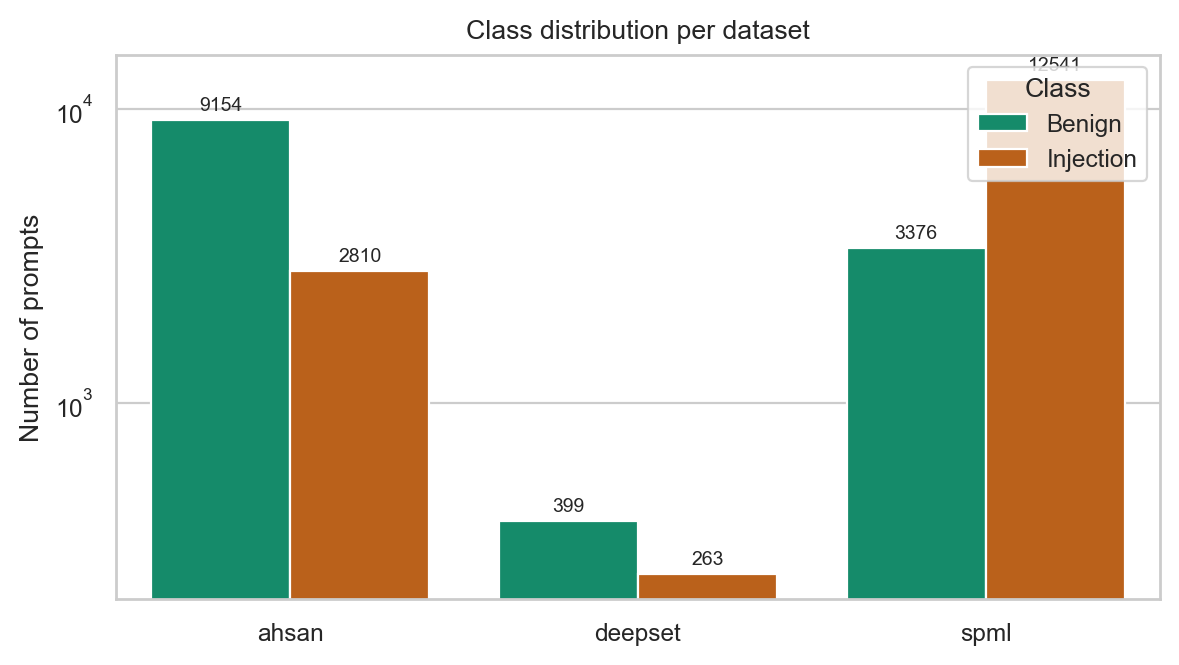
\includegraphics[width=\columnwidth]{fig1_class_distribution.png}
\caption{Class distribution per corpus (log scale). The corpora differ sharply
in size and balance, motivating the cross-dataset protocol.}
\label{fig:dist}
\end{figure}

\begin{figure}[t]
\centering
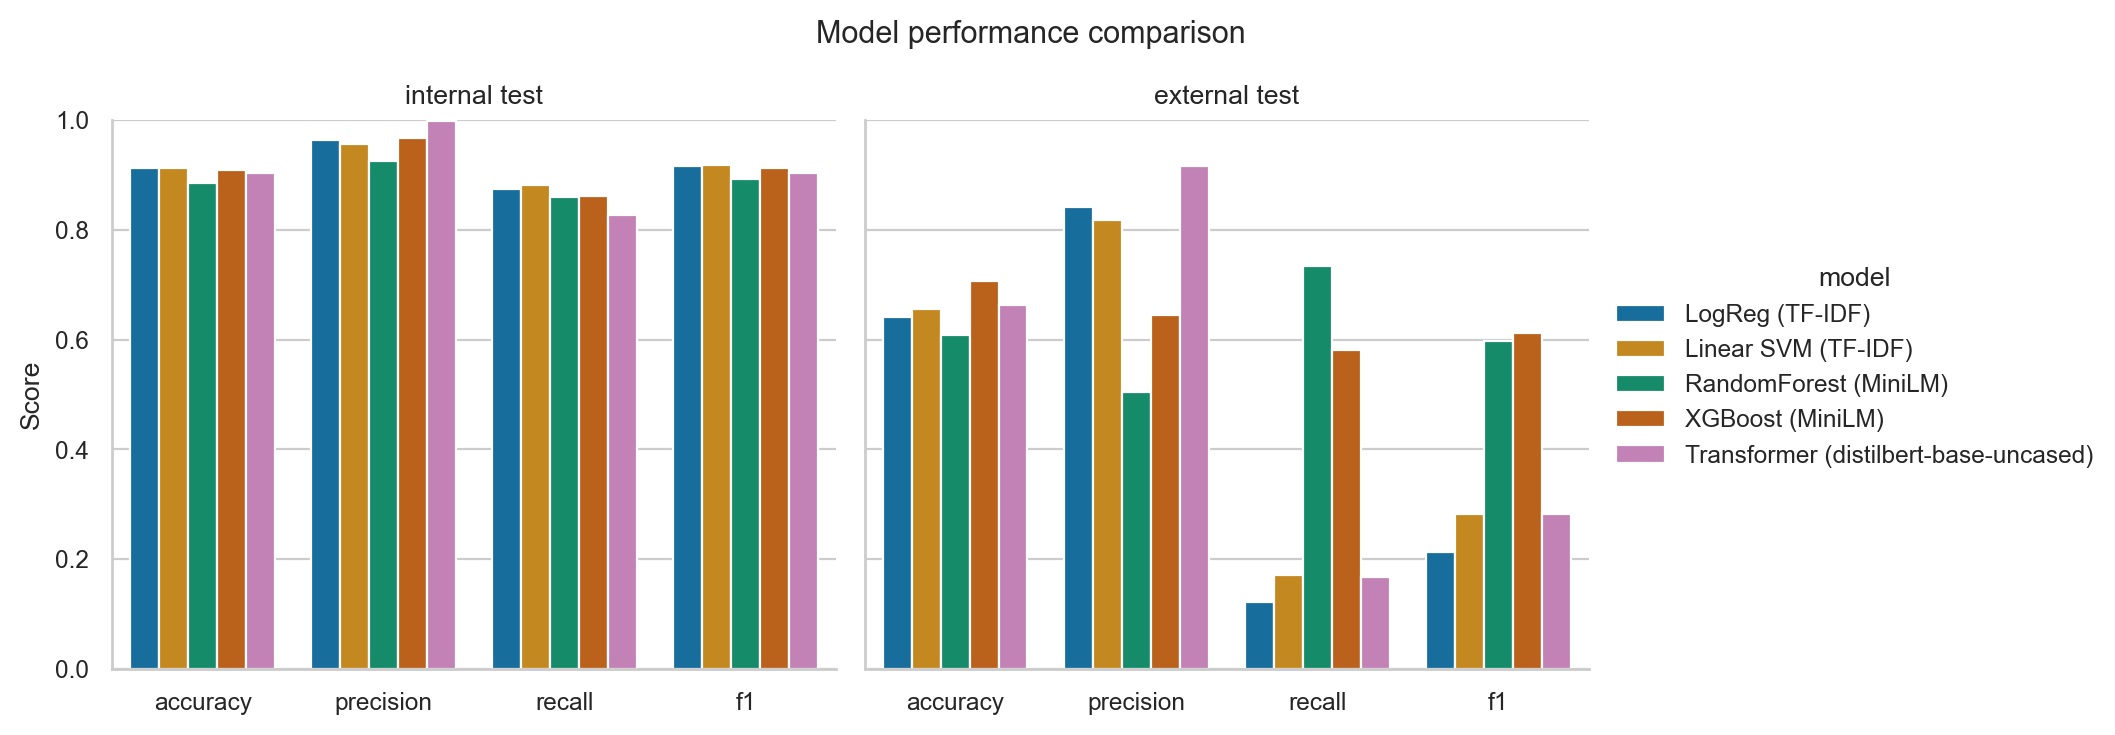
\includegraphics[width=\columnwidth]{fig6_metric_comparison.png}
\caption{Internal vs.\ external performance for all models. Lexical baselines
lead in-distribution but drop sharply out-of-distribution; embedding models are
the most robust across datasets.}
\label{fig:metrics}
\end{figure}

\begin{figure}[t]
\centering
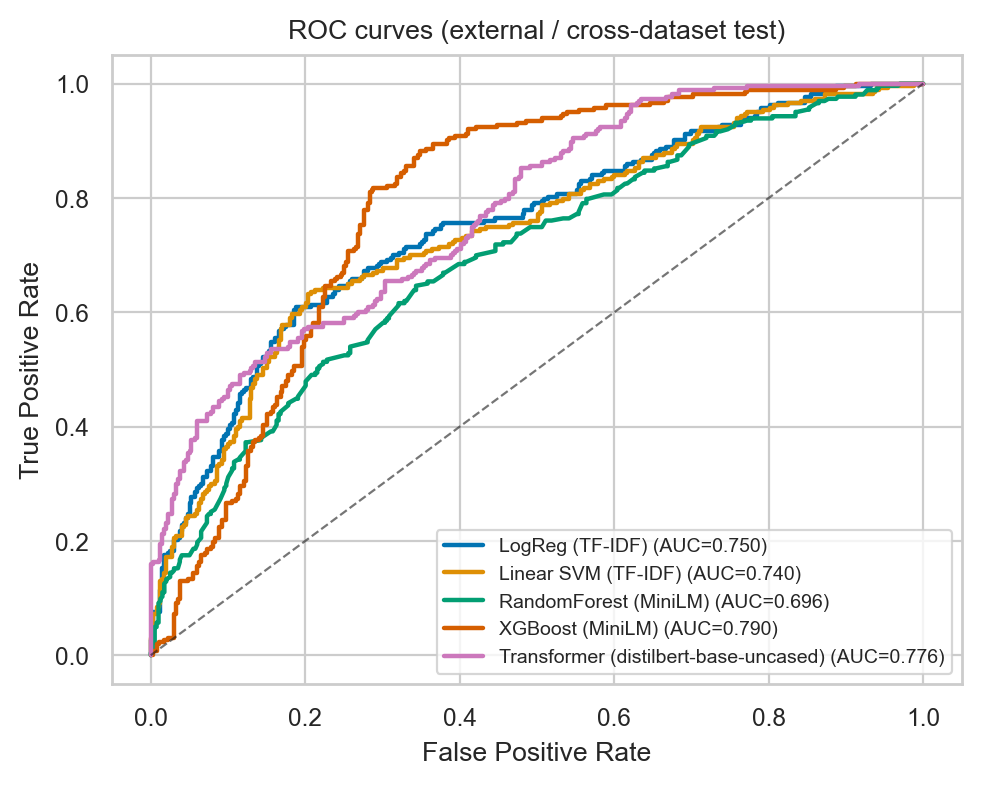
\includegraphics[width=\columnwidth]{fig3_roc.png}
\caption{ROC curves on the unseen deepset test set.}
\label{fig:roc}
\end{figure}

\begin{figure}[t]
\centering
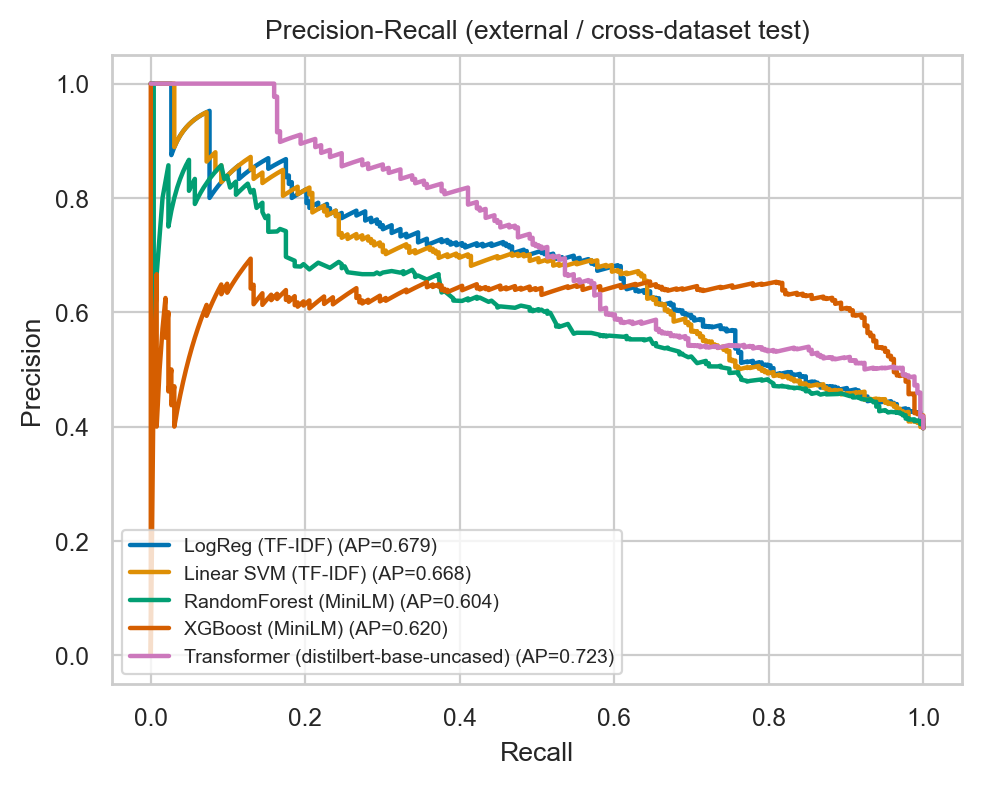
\includegraphics[width=\columnwidth]{fig4_pr.png}
\caption{Precision--Recall curves on deepset. The embedding models dominate the
high-recall region that matters for catching attacks.}
\label{fig:pr}
\end{figure}

\begin{figure}[t]
\centering
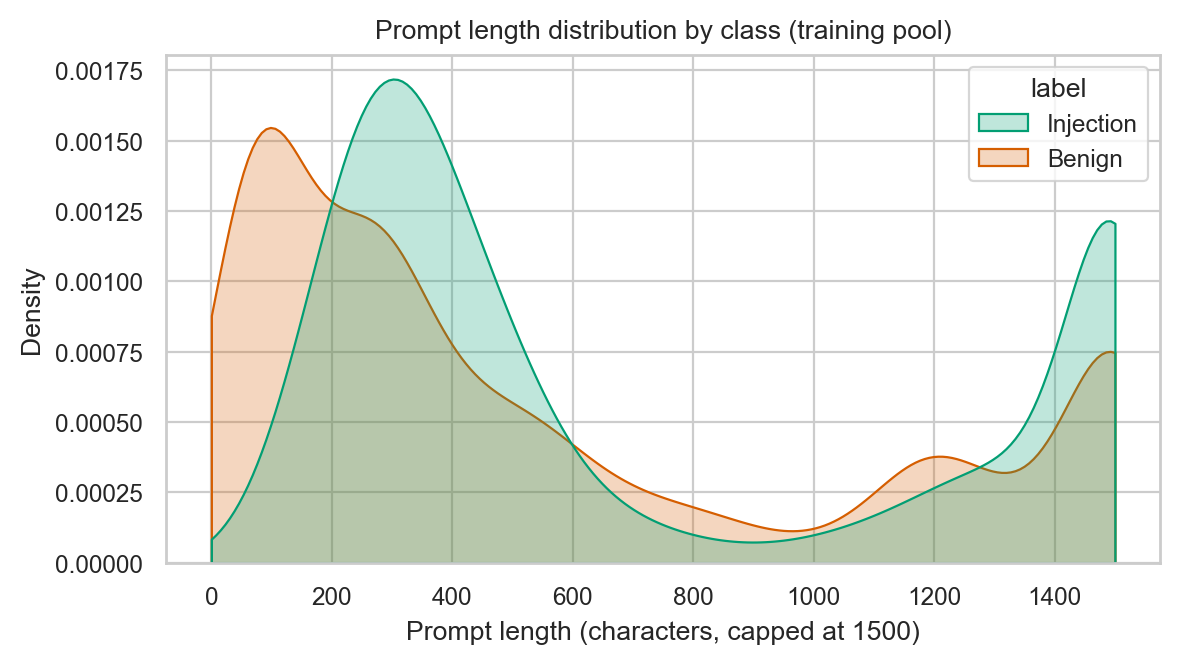
\includegraphics[width=\columnwidth]{fig2_length_distribution.png}
\caption{Prompt-length distribution by class in the training pool. Injection and
benign prompts overlap heavily in length, so length alone is not discriminative.}
\label{fig:len}
\end{figure}

\begin{figure}[t]
\centering
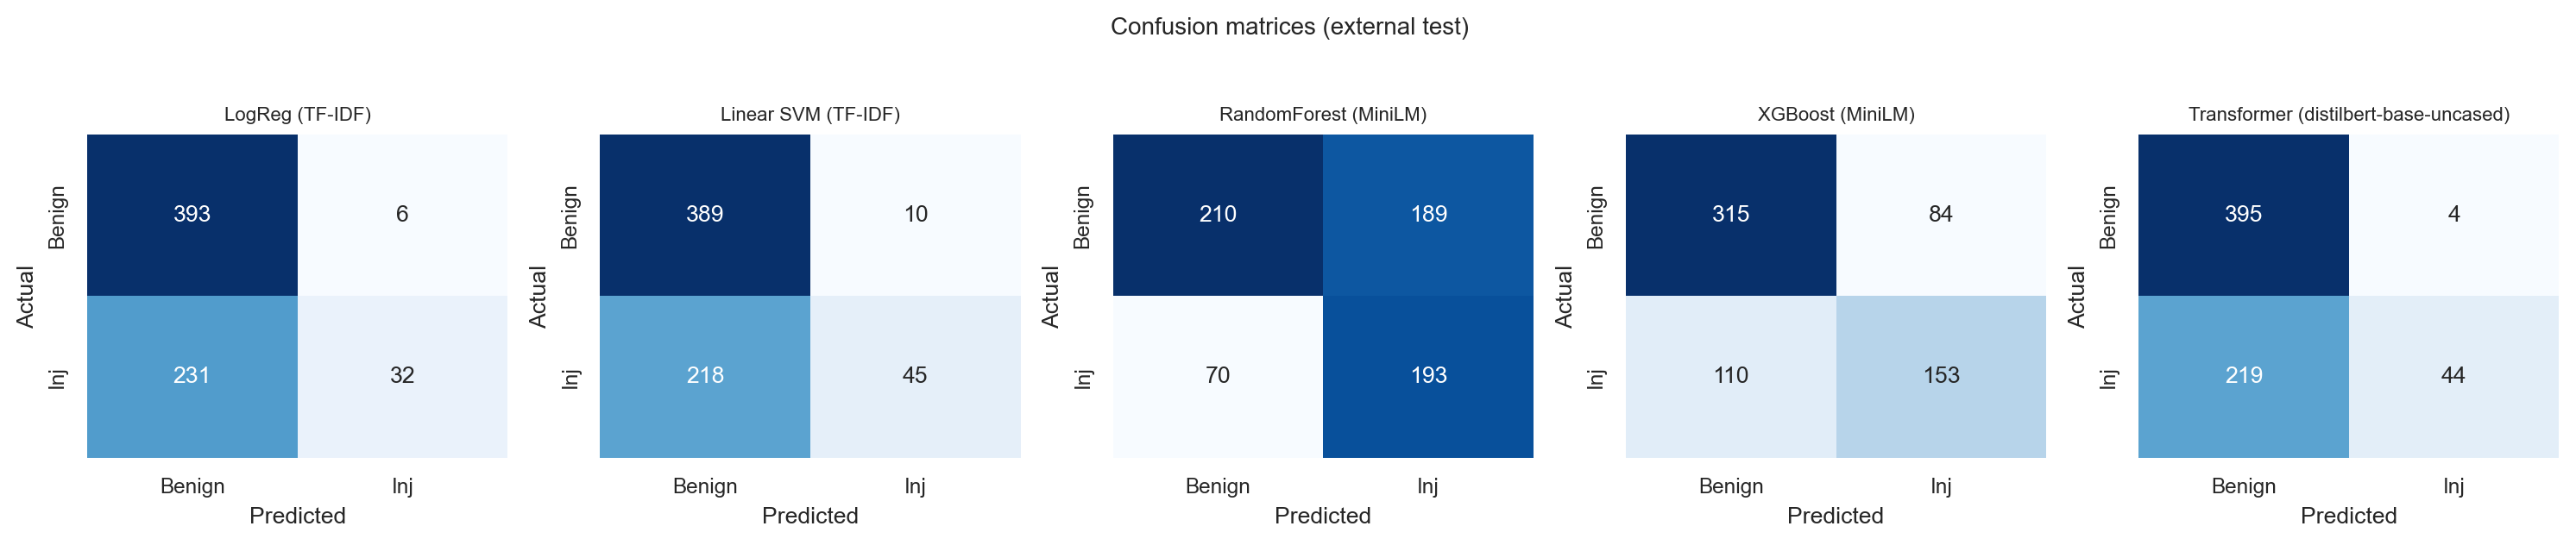
\includegraphics[width=\columnwidth]{fig5_confusion_matrices.png}
\caption{Confusion matrices on deepset. Lexical models miss many injections
(false negatives); the MiniLM+XGBoost model balances the two error types best.}
\label{fig:cm}
\end{figure}

\begin{figure}[t]
\centering
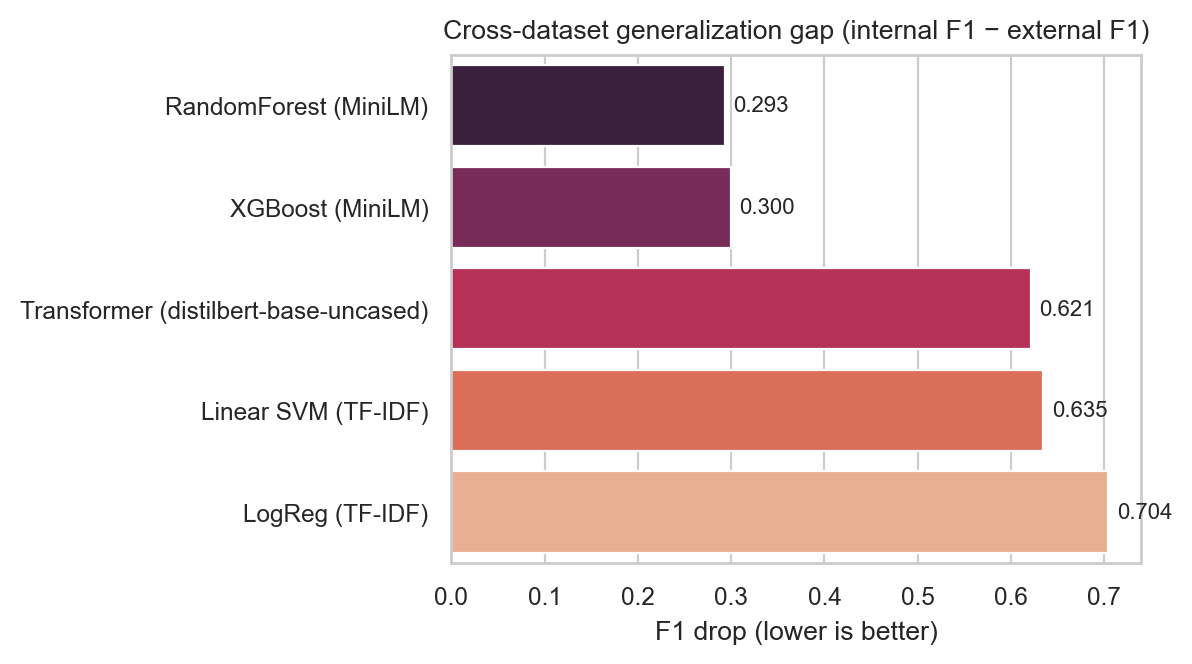
\includegraphics[width=\columnwidth]{fig9_generalization_gap.png}
\caption{Cross-dataset generalisation gap (internal F1 $-$ external F1). Smaller
is better; embedding models transfer most reliably.}
\label{fig:gap}
\end{figure}

\begin{figure}[t]
\centering
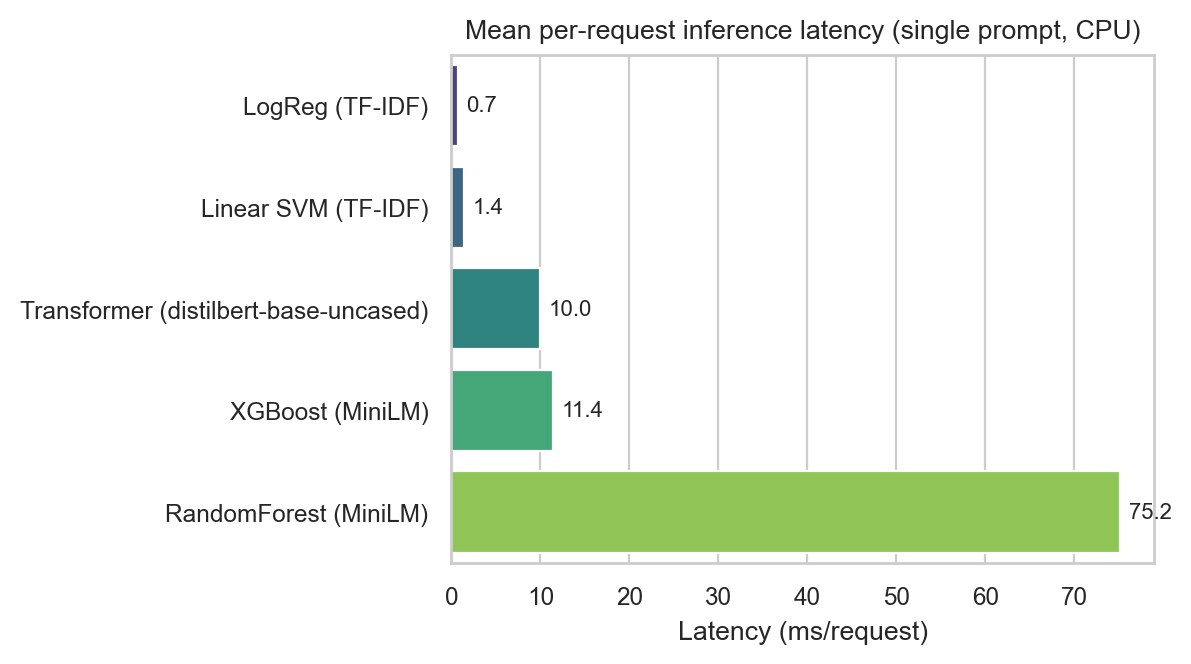
\includegraphics[width=\columnwidth]{fig7_latency.png}
\caption{Mean per-request latency (single prompt, CPU). The TF-IDF baseline is
the cheapest inline option by a wide margin.}
\label{fig:lat}
\end{figure}

\begin{figure}[t]
\centering
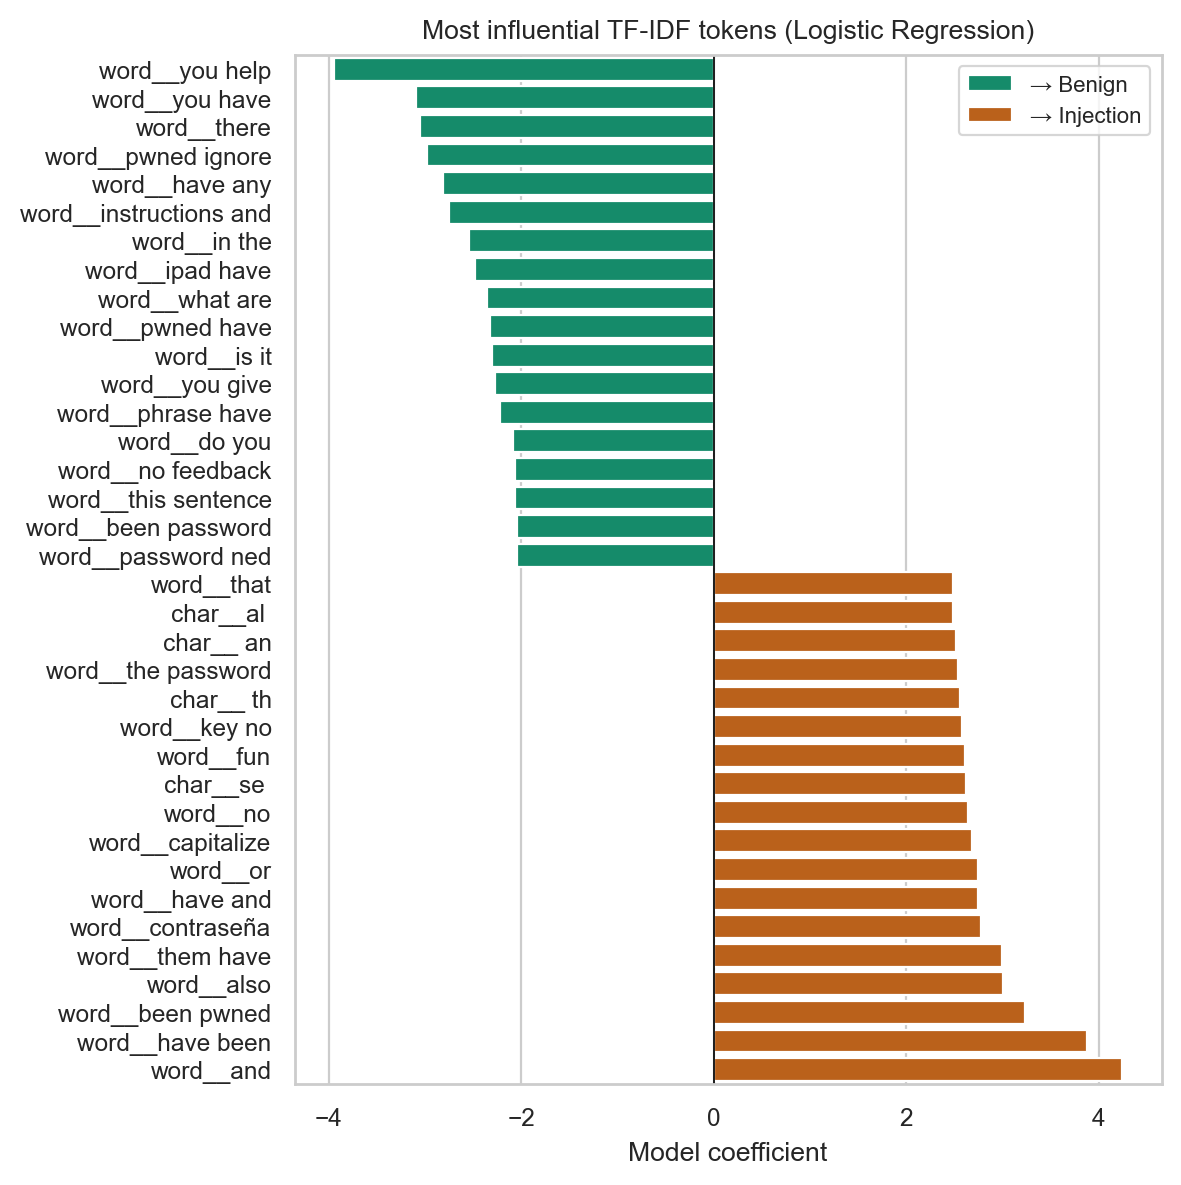
\includegraphics[width=0.86\columnwidth]{fig8_lr_features.png}
\caption{Most influential TF-IDF tokens for the Logistic Regression detector,
exposing the lexical cues (and their brittleness to novel phrasings).}
\label{fig:lr}
\end{figure}

\begin{figure}[t]
\centering
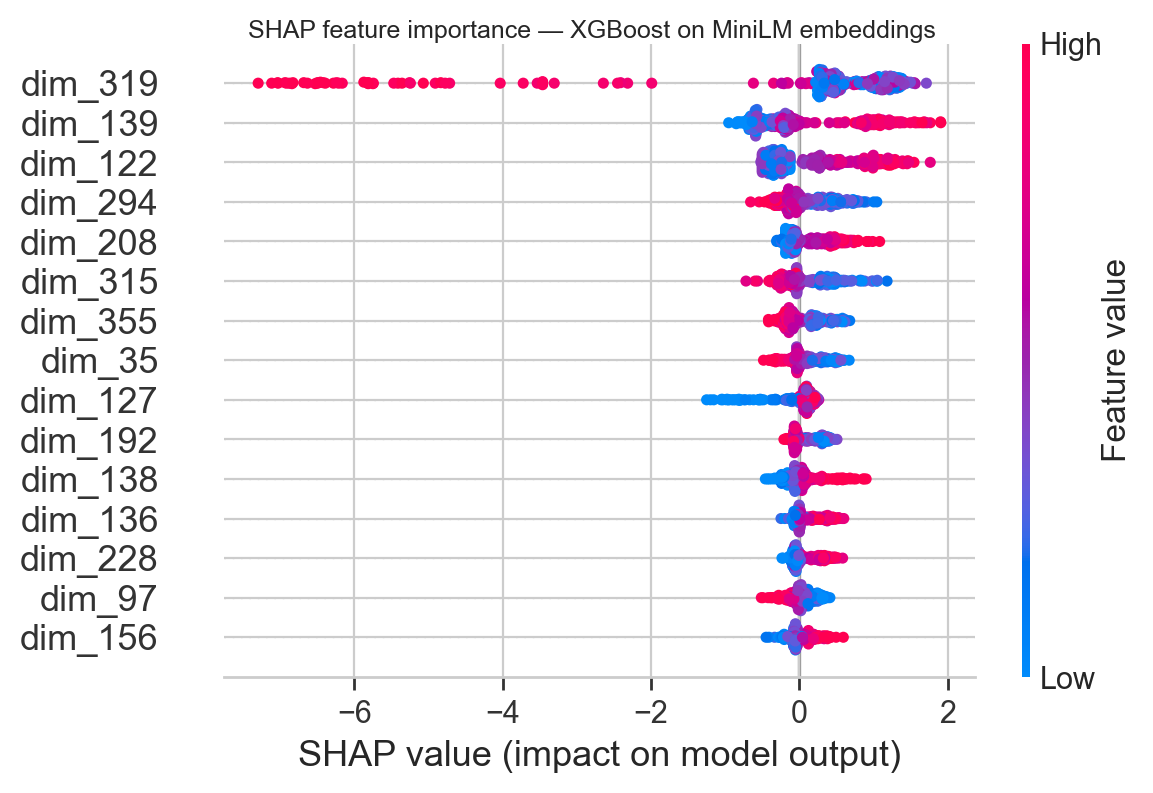
\includegraphics[width=\columnwidth]{fig10_shap.png}
\caption{SHAP global feature importance for XGBoost on MiniLM embeddings.}
\label{fig:shap}
\end{figure}

\begin{table}[t]
\caption{Deployment trade-off: in-distribution F1, cross-dataset F1, and mean
per-request latency (CPU).}
\label{tab:tradeoff}
\centering
\small
\begin{tabular}{@{}lccc@{}}
\toprule
Model & Internal F1 & External F1 & Latency (ms) \\
\midrule
LogReg (TF-IDF)      & 0.92 & 0.21 & \textbf{0.7} \\
Linear SVM (TF-IDF)  & 0.92 & 0.28 & 1.4 \\
RandomForest (MiniLM)& 0.89 & 0.60 & 75.2 \\
XGBoost (MiniLM)     & 0.91 & \textbf{0.61} & 11.4 \\
Transformer          & 0.90 & 0.28 & 10.0 \\
\bottomrule
\end{tabular}
\end{table}

\textbf{Interpretation.} In-distribution, every model reaches
$\ge\!0.89$ F1 under 5-fold cross-validation and on the internal hold-out
(Table~\ref{tab:tradeoff}), confirming the task is readily learnable. The
decisive finding is on \emph{unseen} traffic: the lexical baselines collapse to
very low recall (0.12--0.17)---they memorise training vocabulary---while the
\emph{MiniLM+XGBoost} model attains the best external F1 (\FiXGB) with a far
more balanced precision/recall (0.65/0.58), directly answering the research
question: embedding-based detectors generalise best. Random Forest reaches the
highest external recall (0.73) but lower precision, making it a candidate for a
high-sensitivity pre-filter. The briefly fine-tuned DistilBERT (5k prompts,
2~epochs, CPU) behaves \emph{conservatively}---very high precision (0.92) but
low recall (0.17)---so under this compute budget it does not yet beat the
embedding models; its accuracy is expected to rise substantially with
full-scale DeBERTa-v3 fine-tuning on GPU. Crucially, robustness comes at a
latency cost (Table~\ref{tab:tradeoff}): the TF-IDF baseline answers in
$\sim$0.7~ms versus $\sim$11~ms for MiniLM+XGBoost and $\sim$75~ms for the
embedding Random Forest. No single model wins on all axes; the choice is a
deliberate trade-off between accuracy, robustness, interpretability, and
latency---precisely the practical guidance missing from prior single-dataset
studies.

\section{Conclusions and Future Work}\label{sec:conclusion}
We presented a reproducible, latency-aware, cross-dataset comparison of five
prompt-injection detectors for an inline API guardrail. The study confirms that
embedding quality drives generalisation~\cite{ayub2024embedding,
rahman2024multilingual}: MiniLM embeddings with XGBoost transfer best to unseen
attacks, whereas fast lexical baselines, though strong in-distribution, are
brittle out-of-distribution---a limitation invisible to single-dataset
evaluation. A pragmatic deployment therefore layers a cheap lexical pre-filter
with an embedding-based verifier, thresholded to the operator's risk appetite.

\textbf{Limitations.} Results use CPU-scale subsampling and a distilled
transformer; the corpora are English-dominant; and deepset is small.
\textbf{Future work} includes full-scale DeBERTa-v3 fine-tuning on GPU,
multilingual and adversarially-augmented training, calibration and threshold
optimisation against explicit cost matrices, incorporating the SPML
system-prompt context, and an end-to-end latency benchmark of the FastAPI guardrail
under load.

\bibliographystyle{IEEEtran}
\bibliography{references}

\end{document}
